\documentclass[12pt]{article}
\setcounter{secnumdepth}{2} 
\title{PubCrawl: A Publication Search Engine}
\author{Frank Li (frankli@mit.edu) \\
Abhishek Sarkar (aksarkar@mit.edu)\\
Manasi Vartak (mvartak@mit.edu)}

\usepackage{graphicx}
\usepackage[letterpaper,margin=1in]{geometry}
\usepackage{palatino}
\usepackage{mathpazo}

\newcommand{\citeseer}{CiteSeer$^\chi$}

\begin{document}
\maketitle

\begin{abstract}
Searching for documents ranked by relevance is a well-studied problem in
information retrieval. In particular, there are frameworks for estimating
relevance as a function of the content of the document and algorithms for
estimating relevance as a function of incoming links. However, further
specialization of these techniques is required to search a corpus of academic
papers. Academic papers are highly structured, lending additional weight to
matches which appear in important sections such as the title or abstract.
Contextual information changes the weight which should be contributed to cited
papers. Here we describe PubCrawl, a search engine built for the ACM Digital
Library. The system allows users to weight the relative importance of matches
in various sections of the documents. We also implement a version of PageRank
over the dataset. We evaluate the system in user studies.
\end{abstract}

\section{Introduction}

A primary source of information for computer science researchers are published
papers from conference proceedings and journals. As the number of papers and
venues increases, the ability to quickly find papers relevant to a given topic
becomes more important. In particular, researchers want search engines which
return important papers.

There are several prominent search engines for academic papers: Google Scholar,
\citeseer, and Microsoft Academic Search. Google Scholar uses a proprietary
algorithm which combines several approaches. However, researchers have
partially reverse engineered it \cite{beel09a, beel09b}. In particular, the
algorithm is biased towards highly cited papers, which should highly rank
important papers in the standard literature. However, the bias will also make
the algorithm miss more recent influential papers. Researchers also uncovered
several weaknesses in Google's automatic processing of documents which could
allow authors to game search rankings \cite{beel10}.

\citeseer\ is primarily an automatic citation indexing system \cite{giles98,
  lawrence99, li06}. The system crawls the web and processes documents which
appear to be academic papers. This approach produces a large corpus of noisy
data, which hurts the performance of its ranking algorithm. Also,
\citeseer\ does not make use of the citation data it processes in its ranking
algorithm.

Microsoft Academic Search is a relatively new search engine designed to compete
with Google Scholar. It too uses a proprietary algorithm which combines several
features, and shows the same weakness to ranking optimization as Scholar.


\section{PubCrawl Design and Implementation}

\subsection{Overview}

PubCrawl is an online search website for the ACM Digital Library built with the
Django web framework. It is backed by a Postgres database which stores metadata
(authors, venues, and citations) and a Lucene search index. The PubCrawl
interface allows users to submit search terms and assign relative weights to
title, abstract, and full text searches and PageRank. Figure \ref{interface}
shows a screenshot of the interface.

\begin{figure}[bt]
  \begin{center}
    \includegraphics[width=\textwidth]{images/interface}
  \end{center}
  \caption{PubCrawl user interface}
  \label{interface}
\end{figure}

\subsection{ACM Digital Library}

The ACM Digital Library is a corpus of over 223,800 academic papers published
in ACM journals or conference proceedings. The data set is in XML format with
rich metadata including citations. Unlike \citeseer, we do not have to do
sophisticated NLP to build a citation graph, increasing the quality of the
resulting graph.

However, because the data set is limited to ACM publications, the citation
graph is highly disconnected. Although the vast majority of the papers
(176,285) are contained in one component, in total there are 45,571 connected
components. Figure \ref{comp-size} shows the size distribution of these
components is heavily skewed. We take special consideration of component size
in our adaptation of the PageRank algorithm. Figure \ref{degree-dist} shows the
distribution of outdegrees in the largest component of the citation graph. As
expected, this distribution follows a power law.

\begin{figure}[p]
  \begin{center}
    \includegraphics[width=5in]{images/component-graph}
  \end{center}
  \caption{Distribution of component sizes in the citation graph}
  \label{comp-size}
\end{figure}

\begin{figure}[p]
  \begin{center}
    \includegraphics{images/degree-graph}
  \end{center}
  \caption{Distribution of outdegrees in the largest component of the citation
    graph}
  \label{degree-dist}
\end{figure}

\subsection{Document scores}

We use Apache Lucene \cite{lucene} to index documents and compute relevance
scores. We build the usual inverted index over the corpus, filtering out
stopwords. The structure of the documents is preserved in the XML corpus, so we
can easily parse titles, subtitles, abstracts, and full text. Lucene supports
multi-field documents, so we index and perform searches on each independently.
We also include various metadata to simplify the implementation of the
front-end.

Lucene uses the Boolean model \cite{lancaster73} to filter documents and the
Vector Space Model \cite{salton75} to score documents. Documents and queries
are vectors with each term a dimension and coordinates equal to tf*idf values.
Then, the relevance of a document to a query is related to the angle between
them (the cosine similarity score). Lucene generalizes the cosine similarity
score in several ways. First, documents are allowed to have multiple and
duplicate fields. Second, Lucene allows index-time boosting of documents and
fields as well as query-time boosting of query terms. Finally, Lucene does not
require every term to appear in hits, instead using a coordination factor to
score documents which contain more terms higher. 

While these features can be exploited to improve the quality of search results,
they also have some unintended side effects. In particular, Lucene's scoring is
biased towards matches in shorter fields due to the way it normalizes even
though fields are boosted equally by default. We investigated using user
inputted weights to boost individual fields within Lucene's scoring mechanism,
but found it as difficult to combine the resulting scores with PageRank as
performing three separate searches and combining four scores.

\subsection{Adapted PageRank}

PageRank is a well-known algorithm for estimating the importance of a web page
as a function of the number of incoming links \cite{brin98, page99}. It is
plausible to extend the algorithm by analogy to academic papers and citations.
We use the iterative algorithm as described but tune the parameters to improve
the quality of the results for the ACM data set. The update rule is:

\begin{equation}
R(p)= n\left(\frac{1 - d}{N} + d\left(\sum_{c \in C(p)}
\frac{R(c)}{D(c)}+E(p)\right)\right)
\end{equation}

where $R(\cdot)$ is the PageRank of a node, $D(\cdot)$ is the outdegree of a
node, $E(\cdot)$ is the score source of a node (needed to converge with
cycles), $C(\cdot)$ is the component containing a node, $N$ is the total number
of papers, $d$ is the damping factor, and $n$ is a normalizing factor.

We set $E$ to a uniform vector with each coordinate equal to $0.1$. This
setting minimizes the PageRank each paper gets for free while still allowing
the algorithm to converge. We set $d$ to the suggested value of $0.85$. This
setting reduces the number of iterations needed to converge by reducing the
amount of PageRank contributed in subsequent iterations.

We found initializing the PageRank of each paper to a constant gave suboptimal
results because the ACM citation graph has a high number of small components.
Papers in these components end with disproportionately high PageRank because
further iterations do not change their initial value very much. Instead, we set
the initial value of a paper's PageRank to $\vert C(p) \vert / N$ or the
proportion of all papers contained in its component.

Figure \ref{pagerank-dist} shows the distribution of PageRanks computed in that
component. This distribution also follows a power law, which is expected given
the distribution of outdegrees.

\begin{figure}[p]
  \begin{center}
    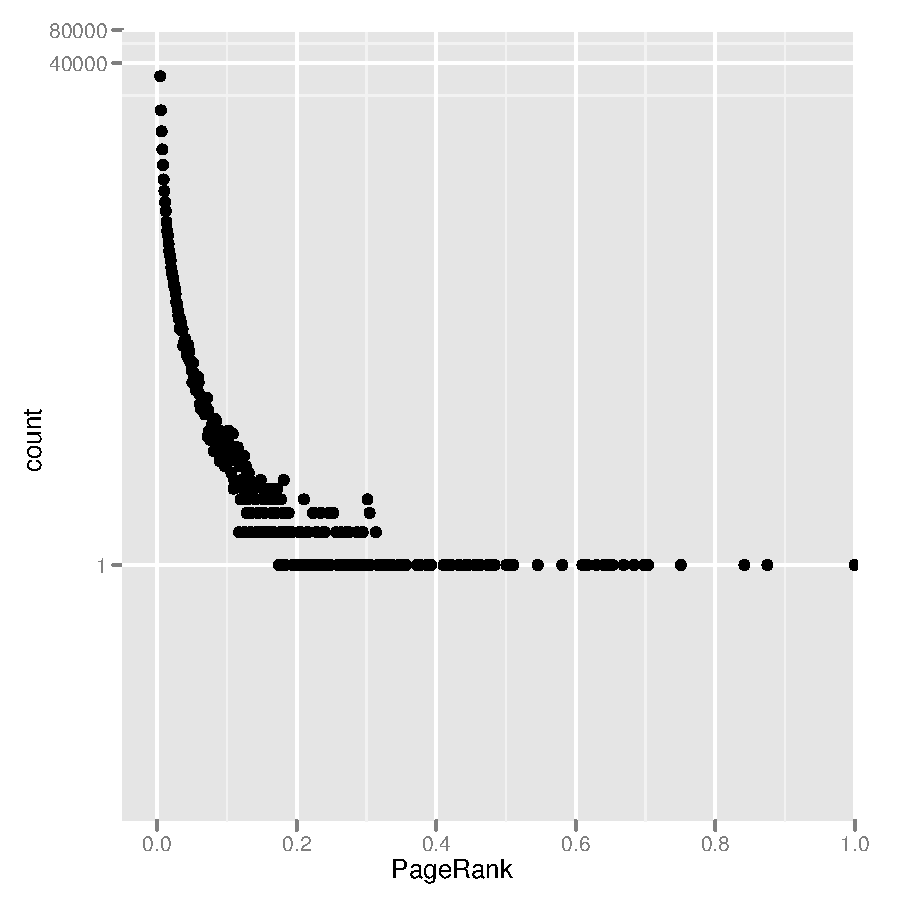
\includegraphics{images/pageranks}
  \end{center}
  \caption{Distribution of PageRanks in the largest component of the citation
    graph}
  \label{pagerank-dist}
\end{figure}

\subsection{Combining document scores and PageRanks}

We compute a final score used for ranking documents as a linear function of
subscores. One issue is that these subscores are not necessarily on the same
scale. In particular, Lucene scores are on an arbitrary scale. To address this
issue, we normalize scores per query.

The PageRank algorithm includes a normalization step at each iteration.
However, if a particular topic is studied by only a few researchers, all the
papers relevant to that topic will have low PageRank. To address this issue, we
renormalize PageRanks per query.

We implemented two ranking functions. The first only uses the full text score
and PageRank. The second uses an algorithm based on RankJoin
\cite{DBLP:conf/vldb/IlyasAE03} to combine lists of hits sorted by each of
title, abstract, and full text scores and PageRank. The algorithm maintains the
top $k$ hits seen so far. In each iteration, we pop the maximum element off of
the next list in round-robin order and hash it. If the element can be joined
with an element seen from each of the other lists, then we update its score in
the top $k$. We special case the list of abstract scores because not all
documents have abstracts. The algorithm terminates when the maximum possible
score of unseen tuples is less than the score of the $k$th hit.

\section{User Study}

\subsection{Methodology}

To evaluate the quality of PubCrawl results, we performed a preliminary user
study comparing the quality of PubCrawl results with those from Google Scholar,
Microsoft Academic Search, ACM Digital Library and \citeseer. We obtained
information from experts about important papers on 6 topics: Provenance, stream
processing, Twitter, crowdsourcing, parallel databases, and NoSQL. We then
manually picked weights shown in Table \ref{weights} that gave good results for
all 6 topics.

\begin{table}[p]
  \begin{center}
    \begin{tabular}{ll}
      Parameter & Weight\\
      \hline
      Title & 0.1\\
      Abstract & 0.01\\
      Document & 0.5\\
      PageRank & 1\\
    \end{tabular}
  \end{center}
  \caption{Manually optimized parameter settings for PubCrawl user study}
  \label{weights}
\end{table}

For the user study, we threw out Provenance and NoSQL from the topics list.
Provenance did not have enough papers in the ACM data set; NoSQL is not a
commonly used term even in papers about such systems. For the remaining topics,
we performed searches on each of the engines, generating lists of the top 10
ACM publications from each. We provided these lists to our experts who rated
each of the 10 results as Highly Relevant, Moderately Relevant or Not relevant.
They also ranked the five lists in order of decreasing quality.

\subsection{Results}

Table \ref{ratios} shows the distribution of relevance of results for each
search engine. Relevant results include both moderately and highly relevant
results. PubCrawl produces a comparable number of relevant documents to the
other search engines. We note \citeseer\ produces a large fraction of
irrelevant documents, which we suspect is due to its noisy data set.

However, PubCrawl produces a relatively low number of highly relevant results.
We believe there are several reasons this is the case. First, our citation
graph does not include non-ACM papers. This means relevant papers may not
necessarily have high PageRank in our system. Second, our Lucene text index
does not index $n$-grams, which reduces the quality of results for multiword
queries. Third, the Lucene scoring function based on VSM has been superseded by
other information retrieval metrics.

Figure \ref{relevance3} shows a quality score for each search engine, defined
as $H - N + .1 M$, where $H$ is the number of Highly Relevant papers, $M$ is
the number of Moderately Relevant papers, and $N$ is the number of Not Relevant
papers.

Figure \ref{rank1} shows the average rank assigned to an engine based on the
ranks assigned to each engine by our experts. A higher score (scale of 5)
indicates a better rank. On average, PubCrawl ranked as high as the other
engines except Google Scholar.

\begin{table}[p]
  \begin{center}
    \begin{tabular}{llll}
      Search Engine & Relevant & Highly Relevant & Not Relevant\\
      \hline
      Google Scholar & 0.9 & 0.45 & 0.1 \\
      Microsoft Academic Search & 0.875 & 0.275 & 0.125 \\
      \citeseer & 0.6 & 0.125 & 0.4 \\
      ACM Digital Library & 0.975 & 0.125 & 0.025 \\
      PubCrawl & 0.95 & 0.1 & 0.075 \\
    \end{tabular}
  \end{center}
  \caption{Ratio of results in each relevance category by search engine}
  \label{ratios}
\end{table}

\begin{figure}[p]
\centering
\includegraphics[width=5in]{images/Relevance3}
\caption{Quality score for each search engine}
\label{relevance3}
\end{figure}

\begin{figure}[p]
\centering
\includegraphics[width=5in]{images/Rank}
\caption{Average ranking of search engines (higher score is better)}
\label{rank1}
\end{figure}

Our preliminary user study only involved 4 topics and hence a larger study must
be undertaken to rigorously study the quality of results. We also observed
that: (1) quality of results depends heavily on the breadth of the search term
(a narrow search term produces better results), (2) ground truth was not always
clearly known, (3) ground-truth is subjective, (4) we had to discard a large
number of highly relevant but non-ACM publications. Furthermore, because we did
not have data for non-ACM papers citing ACM papers, our PageRank algorithm was
weaker compared to other search engines. However, we did show that PubCrawl can
find relevant documents and effectively trade off PageRank and text indexing
scores.

\section{Conclusion and Future Work}

In this work, we built a publication search engine based on the PageRank
algorithm and the Lucene text index. We adapted PageRank for the specific
properties of the citation graph and indexed various paper attributes such as
title, abstract and full text. We then explored multiple ways of combining the
text indexing scores with PageRank. We observed that it is very difficult to
find a scoring function that works well for all search queries. We also
realized that combining scores from orthogonal metrics like PageRank and text
indexing may not be the best method to obtain an overall ranking. Our user
study demonstrates that PubCrawl has a low false positive rate and produces a
large number of moderately relevant results. However, it produces a low number
of highly relevant results and there is potential to extend this work by
finding better ranking functions.

We observed that it is very difficult to find a scoring function that works
well for all search queries. We also realized that combining scores from
orthogonal metrics like PageRank and text indexing may not be the best method
to obtain an overall ranking.

Several extensions of this work are possible. An extremely challenging question
we would like to answer is what is the best way to determine appropriate
weights in a ranking function. Using labeled data points and curve fitting or
SVMs, we are likely to get a better set of results. We would also like to
investigate the following heuristics further: it would also be interesting to
extend page rank so that it takes into account relationships between papers,
i.e. paper A supports paper B, paper A refutes paper B etc. Similarly we would
like to use metadata such as paper venues in order to further refine the
scoring. We also looked into whether we could classify papers based on the
level of expertise a paper expects. This may also be used to boost our search
results.

\section{Acknowledgments}

We acknowledge James Cowling, Adam Marcus, Eugene Wu for their assistance with
the user studies and Sam Madden for his feedback on our methods.

\bibliography{refs}{}
\bibliographystyle{acm}

\end{document}
